
\chapter{磁场}
\minitoc[n]
\section{教学要求}
关于电学的知识,在本书第二册中讲了电场和稳恒电流
的知识,在这册书中讲解磁场、电磁感应以及电磁场的知识。
本章研究磁场以及磁场对电流的作用、磁场对带电粒子的作
用。这些内容是电学的重要组成部分,也是学习电学后几章
内容的基础。

本章教材分三个单元,第一单元包括第一节到第六节,
是在复习初中的磁场知识基础上进一步阐明磁现象和电现象
的统一性,介绍描述磁场的基本物理量--磁感应强度B.第
二单元包括第七节到第九节,讲述磁场对电流的作用力及其
在电表上的应用,第三单元包括第十节到第十三节,讲述洛
仑兹力及其在科学技术中的一些应用。

教材在复习初中学过的有关知识的基础上,要求学生了
解磁极和磁极之间,磁极和电流之间,电流和电流之间的相互
作用都是通过磁场来传递的,从而使学生认识磁场是客观存
在的物质。还要使学生了解,磁场可以用磁力线形象地描
述。在教学中应加强安培定则的练习,使学生能够利用这个
定则判断磁场的方向。

介绍磁现象的电本质,是为了使学生了解电流的磁场和
磁铁的磁场有着共同的起源。为了使学生确信运动电能够
产生磁场,教材介绍了罗兰实验。但在教学中不要求做这个实
验,也不要求对实验的细节加以讨论。教材介绍了分子电流,
但不要求对分子电流是如何形成的作深人的探讨。

磁感应强度描述了磁场的性质,是本章教材的重点内容。
由于这个概念比较抽象,它也是教学上的一个难点。教学中,
为使学生对磁感应强度有个基本认识,可在演示磁场对电流
的作用力的基础上,引出$F$与$I\ell$成正比的关系,再给出磁感
应强度的概念。

介绍直线电流磁场的公式,是为了使学生知道直线电流
磁场的磁感应强度大小跟什么因素有关系,使学生对这种磁
场有具体的了解,不要求学生用公式进行定量的计算。
安培力和洛仑兹力表示磁场对电流和运动电荷的作用,
是电学中的重要规律,因此它们是教学的重点。为了使学生
顺利学好后续课程,应该做好左手定则的练习,使学生掌握好
安培力和洛仑兹力方向的判定。

带电粒子在匀强磁场中的运动在实际中有广泛的应用,
是学习荷质比、质谱仪、回旋加速器等知识的基础。为使学生
理解这一知识,复习好有关的力学知识是个关键。带电粒子
做匀速圆周运动的轨道半径公式和周期公式,要求学生能够
理解公式的物理意义,而不要求学生记忆这两个公式(由于这
两个公式推导过程所用的知识都是他们已经学过的,只要理
解推导过程,推出公式并不困难)。

荷质比的测定和质谱仪、回旋加速是洛仑兹力的具体
应用。要求学生了解测定荷质比的原理及其意义。在质谱仪
和回旋加速器的教学中,主要介绍它们的原理。

由于高中阶段所介绍的有关磁场知识,如磁感应强度、磁
通量、安培力、洛仑兹力等都是通过分析、推理和定量推导才
得出的,因此,教材具有一定的难度。这就要求教师要尽量做
好演示实验,尽量增加学生的感性知识。还要注意讲清分析
问题的思路,使学生能够理解学的内容。

本章的教学要求是:
\begin{enumerate}
\item 理解磁场和磁力线的概念,能运用安培定则确定直线
电流、环形电流以及通电螺线管的磁场的方向。
\item 了解磁现象的电本质和磁性材料的应用.
\item 理解磁感应强度和磁通量的概念.了解匀强磁场的
特点。了解直线电流磁场的磁感应强度的计算公式。
\item 掌握计算安培力的公式和判断安培力方向的左手定
则,了解匀强磁场对平面通电线圈的作用和磁电式仪表的工
作原理。
\item 掌握洛仑兹力的计算公式,理解带电粒子在磁场中做
匀速圆周运动的道理,了解质谱仪和回旋加速器的工作原理。
\end{enumerate}

\section{教学建议}
本章教材的中心是研究磁场的特性及有关的规律,因此
磁感应强度$B$是本章的中心概念,教学时,首先研究磁场的
形象化描述,引出磁力线的概念。然后给出磁感应强度$B$的
概念,并以此概念来展开全章教材,依次讲述磁场对电流和运
动电荷的作用力的规律及其在实际中的种种应用。这样围绕
着磁感应强度$B$这个中心概念,形成了本章的知识结构。

\subsection{磁场及描述磁场的物理量}

从第一节到第三节教材,大部分内容学生在初中均已
学习过,可以在课堂上或在课前要求学生自己阅读课文。教师
在课堂上应做好以下几个演示实验:
\begin{enumerate}
\item 磁极对磁极的作用;
\item 电流对磁极的作用(即奥斯特实验);    \item 磁极对电流的作用;
\item 电流对电流的作用。磁力线的演示,可根据学生情况决定
是否需要做。
\end{enumerate}
在观察实验现象和自己阅读课文的基础上,引
导学生思考和讨论以下几个问题:
\begin{enumerate}
\item 在什么条件下可以在空
间出现磁场?    \item 在四个实验中,各种互相作用的实质是什么?
\item 磁场的方向是怎样规定的?    \item 安培定则的内容是什么?   
 \item 
磁场的起源是什么?其根据是什么?
\end{enumerate}
总之,要用问题来激发
学生思维,尽量调动学生的学习积极性,在上述问题讨论基础
上,根据学生所反映的问题,教师的讲授应着重明确以下
几点:

\paragraph{磁场的起源}
教师通过对罗兰实验的分析和讲解,
明确运动电荷是磁场的起源,从而使学生了解电流周围空间
的磁场和磁体周围空间磁场具有相同的起源。

讲授这个内容的顺序可以这样安排:首先根据奥斯特实
验明确电流是磁场的起源,然后提出磁体的磁场是否也是由
电流引起的问题,教师对安培提出的分子电流的假说进行
介绍,并且进一步说明这个假说完全符合近代原子的电结构
学说(顺便对学生解释一下“假说”是一种推动科学发展的重
要思维方法)。其次根据电流是由电荷的运动形成的,那么能
否直接证明静止电荷一旦运动起来就会产生磁场呢?这时教
师再提出罗兰实验,进行介绍和分析。罗兰实验在中学很难
做成,不要求演示,但必须把这个实验的原理和结果给学生讲
清楚。

\paragraph{磁场力问题}
磁场对电流运动电荷要产生磁场力的
作用,是一个实验事实,必须使学生深刻认识它的重要意义。
磁极之间、磁极与电流之间、电流与电流之间的相互作用都是
通过磁场来传递的。也就是说都是通过磁场对电流产生磁场
力来实现的。教师可以重点讲授电流之间的相互作用,使学
生理解上述观点.如果给平行的两根直导线分别通以电流$I_1$,
和$I_2$, 由于电流$I_2$处于电流$I_1$形成的磁场中,因而受到$I_1$
的磁场的磁场力作用.同样,电流$I_1$处于电流$I_2$的磁场中,
因而受到$I_2$的磁场力作用.所以电流$I_1$和$I_2$之间表现出
的互相吸引或排斥,是通过它们的磁场而间接发生相互作
用的。

\paragraph{磁场的方向}
所谓磁场方向,实质上是指磁感应强
度的方向,这和电场方向是指的电场强度方向相类似。在磁
感应强度概念没有提出之前,应介绍根据磁场力的特性对磁
场方向的规定:在磁场中,探测磁针的$N$极受的磁场力方向
即磁场中该点的磁场方向。这种规定比利用磁场对电流或运
动电荷的作用判定磁场方向要具体和简便得多,有利于磁力
线概念的引入。

要明确向学生指出磁力线是一条闭合的曲线,能够形象
地描述磁场的强弱和方向,磁力线并不是一种客观存在的线。
磁力线上所画的箭头,表示的是磁力线的流向,而不代表磁场
方向。磁力线上任一点的切线方向才是该点的磁场方向。如果
已知磁力线的流向,根据上述方法可确定磁场方向。电流方
向和磁力线方向之间有确定的关系,电流方向变化其磁力
线方向也随之改变,安培定则是记忆和判断这种关系的方
法。安培定则是初中学习过的知识,但仍然要通过一些例题
的练习,使学生熟练掌握,这对于后续知识的学习是十分
必要的。

\subsubsection{磁感应强度和磁通量}
磁感应强度概念的建立是本章的重点.可用类比方
法讲述,即从电场强度概念的建立引入建立磁感应强度概念
的必要性。使学生明确磁场中某点磁感应强度的强弱可通
过一个检验电流在该点受的磁场力的大小来描述。建议按以
下步骤来安排教学:

通过演示实验使学生认识磁场对电流的作用力的零
值条件和最大值条件,即当电流方向和磁场方向平行时(夹
角为$0^{\circ}$或$180^{\circ}$),磁场力为零;当电流方向和磁场方向垂直
时,磁场力具有最大值;当电流方向和磁场方向斜交时,磁场
力介于零值与最大值之间。进而引导学生了解在研究磁场的
强弱时,只有用磁场力的最大值进行比较,才能有确定的
意义。

引导学生分析磁场力的最大值的决定条件。首先使
学生认识在同一个磁场中某处的两根长度相同的直导线上通
以相同电流,因条件完全相同,两根导线受的磁场力的最大值
必然相等。如果将此两直导线并联起来,并保证每根线通过的
电流不变,则两根直导线受的磁场力最大值是一根直导线受
力的两倍,由此可得:$F_{\text{最大}}\propto I$, 如果将此两根直导线串联起
来,并将它们全部置于磁场中,则整根导线受力也是一根导
线受力的两倍,由此可得$F_{\text{最大}}\propto \ell$. 将上述两个结论合并可得:
\[F_{\text{最大}}\propto I\ell\]
可见,对磁场中某处$\dfrac{F_{\text{最大}}}{I\ell}$
是一个恒量,使学生认识到这个恒量可用来描述磁场的强弱,因此给这个比值取名
叫磁感应强度。在这里可向学生指出,电场强度的定义也是
利用电场力与电荷电量的比值。用比值定义物理量是物理学
经常采用的方法。使学生了解这一点对于掌握物理概念是十
分有用的。根据磁感应强度的定义
式$B=\dfrac{F_{\text{最大}}}{I\ell}$,
使学生了解$B$
的单位,并向学生明确$B$是矢量,要指出$B$的方向就是磁场方
向,即磁针的$N$极受的磁场力方向,还要指出$B$的方向和$F_{\text{最大}}$
的方向是不同的,对这一点可让学生讨论练习二2来加深认
识。还应诉学生,$B$矢量完全遵从平行四边形法则,可以进
行合成或分解。在这里还应对匀强磁场的特点作一些介绍。

磁通量是一个重要物理量.在下一章讲电磁感应现
象时,它是描述电磁感应规律的基本概念。首先要根据教材
要求将磁通量的定义呈现给学生。使学生正确理解定义式
$\phi=BS$. 对物理概念要抓住定义式来理解是十分重要的,其
次要从磁力线角度来形象说明磁通量的物理意义。第三,要
讲清$\phi=BS\cos\theta$这一公式,可提出“如果所取的平面与$B$
方向平行时则通过此平面的磁通量为多少?”的问题来研究,
这个问题用磁力线能够很形象地说明,因为没有磁力线通过
该平面,所以磁通量为零。然后再讨论“如果平面面积$S$与$B$
方向既不平行又不垂直时磁通量应如何计算”的问题。因为通
过面积$S$的磁力线条数等于通过面积$S$在垂直于磁力线方向
的投影平面$S_n$上的磁力线的条数,又根据磁通量的定义式可
得$\phi=B\cdot S$, 设平面$S$与$S_n$的夹角为$\theta$, 即$S_n=S\cos\theta$, 则
$\phi=B\cdot S\cdot\cos\theta$. 最后介绍磁通量的单位及磁通密度的概念.

\subsubsection{直线电流的磁场}

这一节教材,是研究直线电流周围磁
场的磁感应强度大小的决定条件。在定性演示实验的基础
上,给出定量公式$B=kI/r$。
可以告诉学生,公式中各量采用国
际单位制时,$k=2\x 10^{-7}{\rm N/A^2}$。
在学过下一节教材后,可指导学
生学习阅读材料,就可以了解$k$值的来源。虽在教学中不要
求学生利用$B=kI/r$
进行计算,但用这个公式来对一些问题
作定性分析,还是必要的,使用公式的条件必须给学生明确
讲清楚。最后,应使学生了解虽然直线电流磁场、环形电流磁
场、通电螺线管磁场的磁感应强度大小的计算公式不同,但均
与电流强度成正比。

\subsection{安培力及其应用}
\subsubsection{安培力的大小}

根据磁感应强度的定义式可得安培
力最大值的计算式为$F=I\ell B$. 本节重点讨论电流方向与磁场
方向不垂直时安培力的计算式.设$I$与$B$的夹角为$\theta$, 我们
以电流方向为基准,把$B$分解为平行于电流方向的分量
$B_{\parallel}=B\cdot\cos\theta$和垂直于电流方向的分量$B_{\bot}=B\cdot\sin\theta$. 由于分
量$B_{\parallel}$对安培力无贡献,即对电流不产生作用力,所以电流受
到的力完全由$B_{\bot}$来决定.则可得$F=I\ell B_{\bot}$, 因而$F=I\ell B\sin\theta$. 
要使学生了解这一公式的适用条件,以及各量的单位。

\subsubsection{安培力的方向}
教学时应通过演示实验,使学生在了
解安培力方向的基础上介绍左手定则。通过实验使学生认识
安培力方向有如下特点:第一,安培力$F$的方向总是垂直于$I$
与$B$所构成的平面,即$F\bot I$和$F\bot B$. 第二,安培力$F$的方向
由$I$和$B$两个量的方向共同决定,如果$I$和$B$其中一个量的
方向变为原来方向的反方向,$F$的方向也就变为原来方向的
反方向。如果$I$和$B$两个量的方都变为原来方向的反方向,
则$F$的方向不变,第三,$I$、$B$、$F$三个量的方向关系如图1.1所
示,可构成三维空间中正交坐标系。在了解上述三个特点之
后提出如何记忆$I$、$B$、$F$三个量的方向关系的问题,可以让学
生思考提出自己的记忆方法,然后介绍左手定则。教学时,
应使学生注意当通电导线与磁场方向斜交时,如何判断安培
力的方向。

\begin{figure}[htp]\centering
    \begin{minipage}[t]{0.48\textwidth}
    \centering
\begin{tikzpicture}[>=latex, scale=1]
\draw[<->](0,3)node[right]{$z$}--(0,0)--(3,0)node[right]{$y$};
\draw[->](0,0)--(-2,-2)node[right]{$x$};
\draw[thick,->](0,0)--(0,1.5)node[right]{$F$};
\draw[thick,->](0,0)--(1.5,0)node[above]{$B_{\bot}$};
\draw[thick,->](0,0)--(-1.5,-1.5)node[right]{$I$};
    \end{tikzpicture}
    \caption{}
    \end{minipage}
    \begin{minipage}[t]{0.48\textwidth}
    \centering
    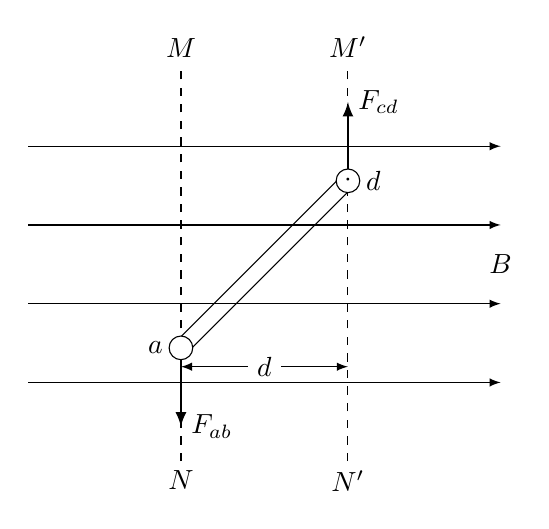
\begin{tikzpicture}[>=latex, scale=1]

\draw[<->](-1.06,-1.3)--node[fill=white]{$d$}(1.06,-1.3);
\foreach \x in {-.5,.5,1.5,-1.5}
{
    \draw[->](-3,\x)--(3,\x);
}      
\node at (3,0){$B$};
\draw[rotate=45](-1.5,-.1) rectangle (1.5,.1);

\draw[dashed](-1.06,-2.5)node[below]{$N$}--(-1.06,2.5)node[above]{$M$};
\draw[dashed](1.06,-2.5)node[below]{$N'$}--(1.06,2.5)node[above]{$M'$};

\node at (45:1.5) [right=3pt]{$d$};\node at (45+180:1.5) [left=3pt]{$a$};

\draw[->, thick](45:1.5)--+(0,1)node[right]{$F_{cd}$};
\draw[->, thick](45+180:1.5)--+(0,-1)node[right]{$F_{ab}$};
\draw(45:1.5)[fill=white] circle (.15);
\draw(45+180:1.5)[fill=white]  circle (.15);
\node at (45:1.5){$\cdot$};
\node at (45+180:1.5){$\x$};
    \end{tikzpicture}
    \caption{}
    \end{minipage}
    \end{figure}

电流天平一节为选讲教材,可在讲完安培力大小和方向
后,把电流天平作为一个实际例子进行介绍。


\subsubsection{磁场对通电线的作用}

可先让学生观察通电线圈
在磁场中偏转或旋转的现象,引导学生分析线圈各边所受安
培力的方向。然后启发学生回忆力偶及力偶矩概念。在此基础
上引导学生定量研究安培力偶矩的大小,再进行分析。在图
1.2中,因$F_{ab}$和$F_{cd}$大小相等、方向相反,又不在一条直线
上,所以$F_{ab}$和$F_{cd}$形成一对力偶。两力作用线$MN$和$M'N'$
之间的垂直距离d为力偶矩的臂。根据力偶矩的定义可得安
培力矩为$M=F\cdot d$, 如是可推导得
\[M=BIS\cos\theta\]

引导学生理解公式时应注意以下几点:
\begin{enumerate}
\item $\theta$角为线圈平
面与磁力线的夹角。如果取线圈平面与中性面(垂直于磁场
方向的平面)的夹角$\alpha$来进行计算,则力偶的臂$d=ad\cdot \sin\alpha$.
因而安培力偶矩为$M=BIS\cdot \sin\alpha$.
\item 如果线圈由$N$匝线圈串
联组成,则$M=NBIS\cos\theta=nBIS\sin\alpha$.
\item 上述安培力偶矩
公式只适用于匀强磁场。
\end{enumerate}

\subsubsection{电流表的工作原理}

首先要使学生明确利用永久磁
铁的磁场使通电线圈偏转的现象制成的仪表叫磁电式仪表,
并通过实物使学生了解电流表的构造。然后重点讲授磁铁与
铁心之间的磁场特点,即磁场是均匀地辐向分布的,就是说所
有磁力线的延长线都通过铁心的中心。不管线圈处于什么位
置,线圈平面与磁力线之间的夹角都是零度。还要明确该磁
场不是匀强磁场,但在以铁心中心为圆心的圆周上,各点的磁
感应强度$B$的大小是相等的。这样,通电线圈受的安培力偶
矩就由下式决定:即$M_1=NBIS$. 电流表内的弹簧产生一个
阻碍线圈偏转的力矩$M_2$. 当$M_1=M_2$时,线圈就停止在某一
偏角$\theta$上,固定在转轴上的指针也转过同样的偏角$\theta$, 并指示
刻度盘上的某一刻度。从刻度的指示数就可以测得电流
强度。

下面再作一些定量的讨论。已知弹簧(游丝)产生的弹性
力矩$M_2$与指针的偏转角$\theta$成正比,即$M_2=k_2\theta$, 其中$k_2$是由
弹簧决定的恒量。由此可得$NBIS=k_2\theta$, 则
\[\theta=\frac{NBS}{k_2}\cdot I\]
从公式得出如下几点结论:
\begin{enumerate}
\item 对同一个电表,$N$、$B$、$S$和$k_2$为不
变的量,则$\theta\propto I$. 可见$\theta$与$I$一一对应,从而可以用指针偏转
角度来测量电流强度$I$的值.
    \item 因为$\theta\propto I$, $\theta$随$I$的变化是
线性的,所以表盘的刻度是均匀的.    
\item 如果$NBS>k_2$, 只要有
很小的电流值,偏转角$\theta$的值就比较大.因此这种电流表的灵
敏度较高. 
   \item 指针最大偏角为$\theta_{\text{最大}}$时,所测得的电流为满偏
电流$I_g$,可得:
\[I_g=\frac{k_2}{NBS}\cdot \theta_{\text{最大}}\]
$I_g$越小,要求$N$、$S$、$B$几个量
都较大。而当线圈的匝数增大时,绕制线圈的导线长度也增
大,则线圈的电阻即电流表的内阻$R_g$增大,可见,灵敏度大
(即$I_g$小)的电流表其内阻$R_g$较大。
\end{enumerate}

\subsection{洛仑兹力及其应用}
\subsubsection{洛仑兹力的大小和方向}

从产生安培力的微观本质
的设想出发,再通过阴极射线管的演示实验来验证这个设想,
使学生获得关于洛仑兹力的感性认识。在此基础上引导学生
推导洛仑兹力公式.推导过程中应抓住以下两点:
\begin{enumerate}
\item 磁场
对电流的作用力(安培力),可看作是作用在每个运动电荷上
的洛仑兹力的合力.这个观点是推导公式的出发点.
\item 引
导学生复习电流公式$I=nqvS$的物理意义。抓住上述两点,按教材思路引导学生得到洛仑兹力大小的公式$f=qvB\sin \theta$.
然后应强调指出$\sin\theta$对$f$大小的影响,即当$\theta=0^{\circ}$时$f=0$, 
$\theta=90^{\circ}$时$f=qvB$为最大值。这些结论对分析运动电荷在磁
场中运动规律是重要的,洛仑兹力的方向仍然用左手定则判
定,要注意讲清洛仑兹力的方向特点。
\end{enumerate}

\subsubsection{带电粒子在磁场中的运动}

没有受到其他力作用的
带电粒子,在磁场中的运动性质是由洛仑兹力来决定的。本
节主要是研究一个带电粒子在匀强磁场中的运动。首先引导
学生思考如果$v$与$B$的夹角$\theta=0^{\circ}$时,带电粒子作何种性质
的运动。然后引导学生重点讨论当$v_0\bot B$时,带电粒子在匀
强磁场中的运动。研究时应抓住以下几点:
\begin{enumerate}
\item 洛仑兹力的方
向永远垂直于含有$v$与$B$的平面,而且由于$v\bot B$, 带电粒子
只能在垂直于磁场的平面内运动。    
\item 由于洛仑兹力的方向垂
直于速度$v$, 所以洛仑兹力不改变速度的大小,只改变速度的
方向。从$f=qvB$公式中可知,如果$q$、$v$、$B$都是恒量,则洛仑
兹力的大小也不变,从中引导学生判断粒子的运动性质,并作
演示实验验证。    
\item 根据带电粒子作圆周运动时洛仑兹力起着
向心力的作用,可得 
\[qvB=\frac{mv^2}{r}\]
进而得出半径公式$r=\dfrac{mv}{qB}$
和周期公式$T=\dfrac{2\pi m}{qB}$
\item 洛仑兹力对运动电荷不做功。这是洛
仑兹力的重要特征.在讲解时还应结合练习七6的讨论,使
学生能利用运动合成、分解的方法,定性地分析带电粒子的运
动方向不和磁感应强度的方向垂直时粒子的运动情况。
\end{enumerate}



\subsubsection{洛仑兹力在近代技术中的应用}

教材中主要介绍质
谱仪和回旋加速器。

\paragraph{质谱仪} 
首先根据课本中质谱仪的装置示意图,介
绍质谱仪的几个主要部件(电离室、加速电场、偏转磁场和显
示器)及其作用,然后推导出荷质比公式
\[\frac{q}{m}=\frac{2U}{B^2r^2}\]

\begin{enumerate}
\item 由于$U$、$B$、$r$均可通过实验测定,因而$q/m$
是微观粒子的基本参量。这
就使学生认识到可运用物理规律设计实验装置,通过宏观量
的测定来测定微观量这样一种重要的物理方法。    
\item 当被测粒
子的电量$q$相同时,在$U$、$B$一定的条件下,不同质量的粒子
在显示器上显示不同的谱线。如果已知电量,则可计算出它
们的质量,质谱仪是十分精密的仪器,是测定带电粒子质量和
分析同位素的重要工具。
\end{enumerate}

\paragraph{回旋加速器}
回旋加速器是利用电场对电荷的加速作用和磁场对
运动电荷的偏转作用来获得高能粒子的装置。可在指导学生
阅读课文后,重点讲清以下几点:
\begin{enumerate}
    \item 使学生了解带电粒子在磁
场中作匀速圆周运动和在电场中作匀加速直线运动的过程。
\item 使学生了解怎样使粒子每次通过电场时速度方向都和电场
力方向相同。主要说明由于带电粒子在匀强磁场中作匀速圆
周运动的周期$T=\dfrac{2\pi m}{qB}$
与速率和半径无关,所以只要交变电
场的变化周期等于粒子的运动周期,就可以使粒子每次通过
电场时都能得到加速。
\item 使学生了解粒子通过$D$形金属扁盒
时,由于金属盒的静电屏蔽作用,盒内空间的电场极弱,所以
运动粒子只受到洛仑兹力的作用而作匀速圆周运动。
\item 设$D$形盒的半径为$R$, 则粒子获得的最大动能为
\[E_k=\frac{1}{2}mv^2_{\text{最大}}=\frac{1}{2}\frac{q^2B^2}{m}R^2\]
可见由于装置的限制,带电粒子在这种加速器中获得的能量也
是有限制的。还要进一步说明,从相对论力学观点来看,粒子
的质量随着速度的增大而增大,这样粒子运动的周期就不再
是恒定的了。因而交变电场的变化周期与粒子运动的周期不
能步,这就使加速器工作条件受到了破坏,进一步提高粒子
的速率也就不可能了。
\end{enumerate}

\section{实验指导}
\subsection{演示实验}
\subsubsection{电流对磁针的作用(奥斯特实验)}



进行这个实验最好自制一个框架,如图1.3所示.底板
可用一长40厘米宽15厘米的厚木板制成,通电导线可用从
旧输电线中拆出的粗单股铜线或铝线,弯成图中所示的形状
固定在底板上,水平长直导线长度约30厘米,高度视所用大
磁针高度而定。接线柱$A$、$B$分别与导线两端相接,接线柱$C$
和$B$相距4厘米,两者之间可接3A保险丝,导线两端经接
线柱$A$、$C$与低压电源直流输出端相连,低压直流电源应选输
出电流大于5A的,例如J1201型教学用低压电源.如无低
压电源,可用4节一号干电池并联后作电源.使用低压电源
时,电压可选2—4V, 此时$B$、$C$间保险丝起限流保护电源作
用.该实验只宜瞬时通电.如果能制作一个如图1.4所示的
大容量电容器充放电装置,利用电容器放电的瞬时大电流,效
果更理想.其中10000 $\mu{\rm F}$ 16V电解电容可用多个电容并联
组成,这个装置还可用于电流间相互作用等实验。

\begin{figure}[htp]\centering
    \begin{minipage}[t]{0.48\textwidth}
    \centering
\includegraphics[scale=.7]{fig/1-3.png}
    \caption{}
    \end{minipage}
    \begin{minipage}[t]{0.48\textwidth}
    \centering
\includegraphics[scale=.7]{fig/1-4.png}
    \caption{}
    \end{minipage}
    \end{figure}

\subsubsection{磁场对电流的作用}
这个实验在初中阶段演示过,若需重新演示,可按以下几
种方法进行。


方法一:按图1.5制作一带有平行金属导轨的底座,导轨
两端与接线柱$A$、$B$相接,用教学演示用的大蹄形磁铁置于导
轨中间,直裸铜线跨搭在两根导轨上,电源可使用供电电流
大于5A的低压直流电源,或用由几节干电池组成的并联电
池组,也可用上一实验介绍的电容瞬时放电装置。同样,这个
实验最好在导线中串有一段3A保险丝以保护电源。如果金
属导轨与直裸铜线所需粗铜线不易找到。可以用从大容量电
解电容器或油浸纸介质电容器中拆出的铝箔制做,把铝箔卷
在细竹棍(毛笔笔杆)上制做导轨。直裸导线则可将铝箔卷在
细竹棍上以后,将竹棍抽出制成。由于铝筒状导线质量极小,
一般用一节干电池即可获得满意效果。

\begin{figure}[htp]\centering
    \begin{minipage}[t]{0.48\textwidth}
    \centering
\includegraphics[scale=.7]{fig/1-5.png}
    \caption{}
    \end{minipage}
    \begin{minipage}[t]{0.48\textwidth}
    \centering
\includegraphics[scale=.7]{fig/1-6.png}
    \caption{}
    \end{minipage}
    \end{figure}

方法二:如想按课本图1.2所示装置进行实验,最好按图
1.6所示将装置改进.图中上方是一根细木条,可固定在铁架
台上。细木条上有两个接线柱,接线柱下固定着铜片。AB是
用铝箔卷成的铝筒,长15厘米左右.与铝筒连接的是两根铝
箔带(宽1.5厘米),使铝筒、铝箔带接触良好,用胶粘牢.铝箔
带上端绕在铜片上两三圈,以保证良好地接触。演示时,用一
节干电池作电源,便可看见通电铝筒在磁场中发生明显偏转。
最好制作两个这样的装置,便于以后演示电流间的相互作用。

若用铜棍与铜导线演示,则应选择能提供5A以上大电流的
低压直流电源,且只宜瞬时接通。

\subsubsection{电流间的相互作用}
由于电流间相互作用力很小,实验所需的大电流(10A以
上)的低压电源又较难找到,在一般学校演示这个实验最好按
下述方法进行。
\begin{figure}[htp]
    \centering
\includegraphics[scale=.6]{fig/1-7.png}
    \caption{}
\end{figure}

方法一:用两条宽2厘米左右的铝箔按图1.7甲所示方
法压制成两条长30厘米的弯曲铝带作平行导线,固定在木架
上,导线间相距1厘米左右为宜(图1.7乙).电源可用6V蓄
电池,通过瞬时短接来获得大电流。注意,只能瞬时短接。如
果利用演示实验1中所述大电容放电装置,效果更好,且不
易损坏电源。

方法二:用演示实验2中所述的铝带与铝筒,将两个这样
的装置平行放置.演示所用电源同上,演示相斥以相距1厘米
为宜,相吸以相距3厘米为宜.以上两个实验若想用低压直
流电源,应选10A输出电流的.实验时,要串一根长4厘米左
右的5A保险丝以保护电源.实验时,仍要瞬时点接。

\subsubsection{磁感应强度的方向}
用十余个小磁针分布在条形磁铁或通电螺线管周围,即
可观察到不同位置的小磁针北极取向不同,表示各点磁感应
强度不同,这个方法简单,但由于只能放在桌面上,因此观察
很不方便。


如果通过投影仪将指南针投影可提高可见度。这需要制
作十余个指向透明的小磁针(图1.8)(可以发动学生在课外
小组活动时制作)。制作方法如下:将磁化的缝衣针(长3厘
米左右)两枚分别对称平行地穿过按扣上的小孔(方法见课本
第364页课外实验活动一“自制指南针”),用透明胶片剪成
箭头与箭尾形状,并分别涂上红绿两色(不能用水彩色或广告
色,可用彩色水笔或照相用的透明颜料),用胶粘在针的两端。
小磁针底座用透明有机玻璃,中间支针可用较粗缝衣针。截取
针尖部分(长1.5厘米),将其烧热后插在有机玻璃底座上,实
验时,将磁针放在投影仪玻璃上,即可在屏幕上看到磁场中透
明磁针南北极的指向。

\begin{figure}[htp]\centering
    \begin{minipage}[t]{0.48\textwidth}
    \centering
\includegraphics[scale=.7]{fig/1-8.png}
    \caption{}
    \end{minipage}
    \begin{minipage}[t]{0.48\textwidth}
    \centering
\includegraphics[scale=.7]{fig/1-9.png}
    \caption{}
    \end{minipage}
    \end{figure}


\subsubsection{通电直导线、环形电流、螺线管磁场的磁力线}
这三种电流磁场的磁力线演示,可以用现成演示仪器
演示,其装置如图1.9、图1.10、图1.11所示.实验电源可用
低压直流电源或6V蓄电池,通过滑线变阻器将电路电流控
制在3—5A间.铁粉最好选用化学实验室中的还原铁粉,也
可用经筛过的细铁屑。实验前,应将铁粉(屑)均匀撒在导线
周围。通电后,轻敲板面,便出现磁力线形状。呈现磁力线
形状后即应断电。

\begin{figure}[htp]\centering
    \begin{minipage}[t]{0.48\textwidth}
    \centering
\includegraphics[scale=.7]{fig/1-10.png}
    \caption{}
    \end{minipage}
    \begin{minipage}[t]{0.48\textwidth}
    \centering
\includegraphics[scale=.7]{fig/1-11.png}
    \caption{}
    \end{minipage}
    \end{figure}

由于环形电流与螺线管磁力线演示器的板面是透明的,
因而可以放在投影仪上进行投影。

以上装置自己制作亦不困难,直线电流磁场磁力线演示
器主要是绕制一个矩形线圈,该线圈可用直径0.3毫米的漆
包线绕制,尺寸为20厘米$\x$20厘米左右,共绕60匝.环形
电流磁场磁力线演示器也用相同直径的漆包线绕60匝左右,
环的直径5厘米左右即可。安放线圈的底座可用有机玻璃制
成(也可用普通窗玻璃条拼接后用胶粘成)。螺线管磁场磁力
线演示器中,螺线管线圈仍用上述导线绕制,每20匝捆扎在
一起,共五组,管直径4—5厘米,间距1.5厘米左右.底座仍
用有机玻璃制作。

如果将这三个装置配以小磁针即可用来验证右手螺旋法
则(安培定则)。


\subsubsection{电流天平}
\begin{figure}[htp]
    \centering
\includegraphics[scale=.6]{fig/1-12.png}
    \caption{}
\end{figure}

J2408型电流天平如课本上图1.28所示,它主要由
激磁线圈(管内产生被测匀强磁场)和横梁系统两部分组成
(图1.12)。激磁线圈内径5.5厘米,匝数约500匝,两端引
线与靠近线圈一侧的接线柱连。横梁系统由铜箔板制成,
中央两侧有黄铜制的刀口并兼作导电接点,铜箔板中央有一
“7”形螺丝,水平部分螺母为横梁平衡螺母.固定在板上竖
直部分下端螺母为配重螺母,用于调节天平灵敏度(越往下,
横梁重心越低,平衡越好,但灵敏度越低)。左侧有一挂钩,
用于悬吊砝码,右侧伸入线圈内部部分铜箔上形成“彐”字形
导体,通过转换开关改变导体在磁场中受力部分(产生力矩部
分)长度为4厘米或2厘米.

演示方法:电流天平主要用来演示一种测量磁感应强度
的方法,即根据定义式$B=\dfrac{F}{I\ell}$测量磁感应强度。演示前
应使天平底座置于水平位置,并调节横梁平衡螺母使横梁平
衡(指针指示中间零刻度),演示时应先接激磁电路。由于激
磁绕组额定电流为3A, 电路中串有3A量程电流表用于监
视.然后再接测量电路.电路连接如图1.13所示,通电导体
长度可根据需要通过转换开关在4厘米或2厘米中选择一个,
通电电流可由串联在电路中的安培计读出,受力大小可通过
悬挂砝码使天平重新平衡的砝码质量求出,需要注意的是,
测量之前应先通电观察一下,不悬挂砝码时指针偏转方向是
否右端(伸入磁场部分)向下,否则应更换测量电路电源极性,
以使电流受力方向改变.由于测量部分额定电流也是3A,因
而实验中电流取值也应限制在3A以下,其次,由于电流天
平配置的砝码只有20毫克、40毫克、60毫克三种,所以在演
示时,调好平衡后,悬挂20毫克砝码,再接通激磁电路,调节
激磁电流,使天平恢复平衡,而后就不需再调,测量对象就是
该激磁电流所产生的磁感应强度。
\begin{figure}[htp]
    \centering
\includegraphics[scale=.6]{fig/1-13.png}
    \caption{}
\end{figure}

这个电流天平还可演示$F\propto I$及$F\propto\ell$的关系,也可演示
激磁线圈内磁感应强度$B$与激磁电流成正比,不再赘述。使
用电流天平前最好用酒精清洗刀口与刀口支承处,以使通电
接触良好,使用后要把横梁从支承架上取下放好,以保护
刀口。

\subsubsection{磁电式仪表的工作原理}
这个实验主要是演示通电线圈在磁场中所受力偶矩和这
个力偶矩与游丝反力偶矩的平衡问题。磁电式仪表的幅向磁
场及完整结构仍需用大幅教学挂图或模型说明。

线圈在磁场中受力偶矩的演示可以用J2416型电机原理
说明器进行,实验装置如图1.14所示.激磁线圈所用电源可
用6V蓄电池或低压直流电源(6—8V),通电线圈电路中串有
变阻器,接在6—8V低压电源或蓄电池上,电路中电流控制
在3A左右为好.
\begin{figure}[htp]
    \centering
\includegraphics[scale=.6]{fig/1-14.png}
    \caption{}
\end{figure}

演示游丝反力矩的作用,需要自制一个教具,其结构包括
磁铁轭、动圈绕组与底座三部分,见图1.15. 制作方法如下:
磁铁轭需要从旧的扬声器(口径4英寸或5英寸,小一些也
可)上拆下钡恒瓷(钡铁氧体)磁体,根据它的大小用2毫米
厚的铁板弯成“凵”形,并用胶把磁体按1.15甲粘在其上,磁
体另一端面粘一块矩形铁片,并使两个磁体$N$、$S$极相对,间
距6—8厘米,动圈绕组用硬泡沫塑料(可从仪器包装中找到)
制成框架,其尺寸根据磁铁轭大小而定,其宽度应尽可能接
近磁铁两极的距离.在框架上用直径0.3毫米漆包线绕20至
30匝,在框架两端中央插入两根粗缝衣针作为转轴,用胶将
线圈与转轴粘牢,线圈头尾部分先分别在前后转轴上紧绕
4—5匝固定后,再弯制成大型游丝状,最后可用按钉将线头固
定在底座木板上。在线框中央立一根用红色油漆涂过的塑料
管作指针,磁铁轭两极也应分别涂上红、蓝两色油漆来表示
$N$、$S$极。底座可用木板制,动圈支架可用薄铁皮或曲别针铁
丝弯制成,底座宽度应恰好卡紧在磁铁轭下部,底座上动圈支
架兼作导电接点,安装两个接线柱便于通电。装好后的仪器
如图1.15乙所示.
\begin{figure}[htp]
    \centering
\includegraphics[scale=.6]{fig/1-15.png}
    \caption{}
\end{figure}

实验时,可先将固定游丝的按钉拔下,使游丝自由。通电
后可以发现,动圈将转至中性面,再固定游丝,通电后可以看
到只转过一定角度。电流越大,偏转角度越大,从而说明了动
圈式磁电仪表的原理。

\subsubsection{带电粒子在磁场中运动时的偏转}
这个实验可以用多种方法进行演示。
\begin{figure}[htp]
    \centering
\includegraphics[scale=.6]{fig/1-16.png}
    \caption{}
\end{figure}

方法一:用JYSI型阴极射线管演示,将一台感应圈与
低压直流电源(或蓄电池)产生高压加在阴极射线管两端。可
以看到在荧光屏上呈现绿色光带,这是电子流撞击荧光屏而
发出的,它表示电子流径迹。当用磁铁靠近射线中部时,阴极
射线将发生偏转,如图1.16所示.反转磁场方向,射线也向
相反方向偏转。这个实验也可以用一般的示磁效应阴极射线
管进行,实验时,如果仅在阴极板附近有绿光而无光带出现,
说明感应圈极性接反,应通过更换极性开关改变极性。

方法二:利用教学示波器荧光屏演示,先将Y增益逆时
针旋到底,Y轴衰减拨至100或1000, 扫描范围拨至外X, X增
益也逆时针旋到底。开启电源后,调节亮度与聚焦,使光点圆
而亮度适中并居于中心,再用磁铁靠近光点,就会发现光点发
生位置变化,根据位置变化与磁极位置就可验证洛仑兹力的
方向与左手定则。
\begin{figure}[htp]
    \centering
\includegraphics[scale=.6]{fig/1-17.png}
    \caption{}
\end{figure}

方法三:利用通电溶液中正负离子受洛仑兹力偏离原来
径迹而带动液体转动来演示.实验装置如图1.17所示,所需
器材在图中均已注明,置于扬声器磁铁上的玻璃培养皿(生
物实验室中常用)的中央部分,置一旧的铜质砝码作为中心电
极,紧靠玻璃培养皿器壁内侧,用紫铜片弯成一个环形电极。
培养皿中倒入比重约为$1.04{\rm g/cm^3}$的硫酸铜溶液,深度为
0.5厘米至1厘米,电流强度由变阻器控制,电流用安培计监
视,一般控制在0.5至0.6安之间,电源可使用低压电源或6V
蓄电池,实验时,在环形电极与中央电极间形成幅向电流。形
成电流的正负离子在洛仑兹力作用下(由于正负离子运动方
向相反,故受洛仑兹力方向一致),带动液体围绕中央电极旋
转,其旋转方向可由左手定则判定,为观察方便,可将培养皿
与磁铁置于投影仪玻璃板上,在液面上撒一些碎纸屑,投影在
屏幕上可使学生清楚看到旋转的液流。若改变电流方向或磁
铁方向就可看到液流反转,从而说明带电粒子在磁场中的受
力及其规律。

\subsubsection{电子束在匀强磁场中作圆周运动}
实验要用磁场、电场作用力演示仪。该仪器目前有两种
规格,即J9283-1型与J9283型.J9283型是改进型,内部附
有电源.J9283-1型内部无电源,需要与J1201型低压电源
(或有9V稳压输出的低压直流电源)及J1205型高压电源
(或有300V高压直流及6.3V交流电压输出的其他高压电
源)配合使用。

此仪器主要由演示球形电子射线管(威尔尼特电子管)与
激磁线圈(亥姆霍兹线圈)组成.J9283型磁场、电场演示仪
外形如图1.18所示.电子管阴极在加热后经加速电压作用
形成电子流射出,充满管内的低压惰性气体在电子流撞击下
将放出紫色辉光,从而观察到电子流的径迹。两亥姆霍兹线
圈互相平行,在两者中央平行平面附近将形成一个匀强磁场
区。电子流在磁场作用下将受洛仑兹力作用,若电子流运动
方向与线圈平面平行,将观察到电子流作匀速圆周运动的径
迹。改变加速电压可改变电子运动速率,改变激磁电流可改变
电子流所处磁场磁感应强度,从而可观察到电子圆运动半径
与电子速度和磁感应强度的关系。
\begin{figure}[htp]
    \centering
\includegraphics[scale=.6]{fig/1-18.png}
    \caption{}
\end{figure}

实验操作步骤如下:
\begin{enumerate}
\item 先将加速极电压旋钮旋至0(逆时
针到底),励磁电流方向旋钮拨至“断路”,幅值旋钮拨至最小
值“0.6A”,偏转板电压钮拨至“断路”(这是用于演示电场偏
转的,此实验中不用偏转电压)。
    \item 接好电源后开启电源,
预热5分钟.
    \item 缓慢调节加速电压旋钮,可以看到电子射线
的紫色直线径迹。用手转动电子管,使径迹与线圈平面平
行.
    \item 拨动励磁旋钮至“顺时”位置,此时,线圈中通有0.6A
励磁电流,其方向由线圈上符号标明为顺时针方向电流(正面
看),此时可看到电子射线径迹发生弯曲。
\item 逐渐加大励磁电
流,可以看到径迹逐渐变为圆形,由此清楚表明运动电子在
磁场力作用下作匀速圆周运动。
\item 继续加大励磁电流(注意,
使用J1201低压电源时,其稳压电流输出不要超过1.2A),由
于磁感应强度增大,电子射线圆径迹半径将减小,说明磁场越
强,圆运动半径越小。
\item 固定励磁电流不变,改变加速电压大
小,将看到电压越高,电子射线圆径迹半径越大,说明磁场不
变时,带电粒子速度越大,其圆运动半径越大,从而定性地说
明带电粒子在垂直磁场方向上运动时,其圆运动半径
$r=\dfrac{mv}{qB}$.
\end{enumerate}

实验时必须注意以下两点:一定要在将加速电压钮逆时
针旋到底再开启电源对灯丝预热5分钟,而后进行实验.实验
完毕后仍应将加速电压钮逆时针旋到底,再关闭电源。其次
在使用励磁线圈电流方向钮时,一定要将幅值钮旋回“0.6A”
处再使用,防止大电流换切造成开关点电弧烧毁接点。

这个仪器还可定量研究验证洛仑兹力规律,亦可配合加
速电压测定电子荷质比,请参阅本仪器有关说明。

实验中若需观察粒子速度方向与磁力线不垂直时出现的
螺旋状径迹,只需用手慢慢旋动电子管即可。

\subsection{学生实验}
\subsubsection{观察磁铁对电流的作用}
这个实验比较简单,最好在课本图10.1所示实验电
路中串入变阻器和安培计。因为现在许多学校已改用低压学
生电源,不再使用蓄电池作为学生实验电源,若采用课本上
的电路,则实际上处于短路状态,往往将保险丝烧断。实验
前,将电路电流调节至2A左右(输出电压4~6V),断开电
键,放好磁铁再进行实验。

在学生进行实验前,教师应作如下要求:首先是弄清
实验原理,即将按左手定则判断导线受力方向的结果与实际
通电后导线受力方向进行比较,这就需要先作出表格(可画
图),其次要求学生观察清楚线圈绕制情况,确定出受力边框
上导线电流流向。

在实验时,可以安排两个思考问题供学生思考:①这
个实验为什么要用多匝线圈代替单根导线进行实验?②有人
说,导线框通电后受磁场力才运动起来,可见力是物体运动的
原因。这种说法对吗?为什么?

\subsection{课外实验活动}
\subsubsection{自制指南针}
最好按前面演示实验4中所介绍的方法制做透明磁针.
磁针底座可改为小木块。安装支持钢针时,可先在木块上用
直径类似的小钉钉一个小孔,再将钢针底部插入固定,并用一
点乳胶粘牢,底座也可用大橡皮,将钢针插在其上便可。

\subsubsection{验证环形电流的磁场}
应让学生弄清线圈绕制方向与电流关系,电流从哪端流
人,怎样在线圈中流动,弄清这一点对后面电磁感应有关线圈
问题和实验很有好处。同时还要告诉学生用砂纸将漆包线两
端漆皮打去,露出铜金属光泽后才能通电,这一点许多学生并
不懂得,实验中所采用的漆包线直径可选用直径0.3毫米左右
的,最好绕30匝左右,通电时间亦不应过长,用低压直流电
源要串一变阻器。

\subsubsection{验证通电螺线管的南北极}
在实验前要指导学生制做螺线管。螺线管直径应大一些,
为使螺线管有一定的形状,需要先用硬卡片纸(或画报纸)制
作一个稍粗的纸质圆筒.绕制时,可用直径0.2—0.3毫米的
漆包线.固定漆包线头尾的方法如图1.19所示,图中的$A$、$B$
是两根粗棉线,待漆包线绕紧后抽紧。螺线管绕制匝数在
30—40匝之间即可.实验时,线头处漆皮也应用砂纸打去,
并且不要长时间通电,以防止损坏电源。用低压直流电源,一
定要加变阻器控制电流强度。
\begin{figure}[htp]
    \centering
\includegraphics[scale=.6]{fig/1-19.png}
    \caption{}
\end{figure}

\subsubsection{观察磁化现象}
注意在做这个实验时,是要把磁铁靠近铁钉。对于实验
现象,可作这样的解释:第一次用磁极一端(如$N$极)靠近时,
铁钉被磁化,靠近磁铁端为异名磁极(如$S$极),吸引铁屑端为
同名磁极(如$N$极)。小铁屑也被磁化,靠近铁钉一侧为异名磁
极(如$S$极)。当移去磁铁时,少量铁屑粘在铁钉上是由于这
部分铁屑都残留有剩磁,其极性不变。当用磁铁另一端(如$S$
极)靠近钉子头的瞬间,由于铁钉磁化靠近铁屑端为同名磁
极($S$极),而铁屑这一端由于原来剩磁磁极未变(还是$S$极),
因而同名相斥而掉落下来了。在解释时,可以向学生说明,铁
钉一般都是熟铁,是软磁性材料,而铁屑成分复杂,即使原
来是软磁性的,由于切削过程的高温,将使内部碳成分集中在
表面,表现出碳钢性质(硬磁性质),这就是铁屑磁化后有些剩
磁较强的原因。


\subsection{练习一}
\begin{enumerate}
    \item 磁体的北极在磁场中所受的磁场力跟磁场方向同向,南极所受的磁场力跟磁场方向反向.课本图1.12是放在磁场中的小磁针,试根据小磁针所受的力说明,它将怎样转动以及静止在哪个方向.
\begin{figure}[htp]
\centering
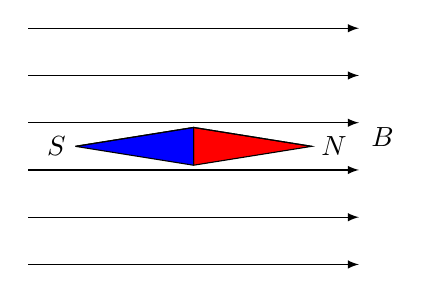
\begin{tikzpicture}[>=latex, scale=.6]
\foreach \x in {-.5,.5,...,4.5}
{
   \draw [->](-2,\x)--(5,\x);
}

\draw [fill=red](2.5-1,-.4+2)--(2.5-1,.4+2)--(5-1,2);
\draw [ fill=blue](2.5-1,-.4+2)--(2.5-1,.4+2)--(-1,2);

\draw (-1,2)node[left]{$S$}--(2.5-1,-.4+2)--(5-1,2)node[right]{$N$}--(2.5-1,.4+2)--(-1,2);
\draw (2.5-1,-.4+2)--(2.5-1,.4+2);

\node at  (5.5,2.2){$B$};
\end{tikzpicture}
\caption{}
\end{figure}




\begin{solution}
    根据磁针$N$极所受的磁
    场力的方向为磁场方向的规定,可知小磁针应顺时针转动。小磁
    针静止在跟磁力线平行的位置上
    (图1.20)。
\end{solution}

    \item 在课本图1.13中,当电流通过导线时,导线下面的磁针北极转向读者.试判断$AB$中电流的方向.


    \begin{solution}
        $AB$中的电流方向由$B$流向$A$.
    \end{solution}
    
    \item 在课本图1.14中,当电流通过线圈时,磁针的南极指向读者.试确定线圈中电流的方向.


    \begin{solution}
        电流沿顺时针方向流动。
    \end{solution}
 

    \item 试确定课本图1.15中电源的正极和负板.


    \begin{solution}
        电源右端为正极。
    \end{solution}
    
    \item 离开你向前运动的质子流产生的磁场是怎样的?向着你运动的电子流产生的磁场又是怎样的?


    \begin{solution}
        磁力线是在垂直于质子速度的平面上,并以质子流为
        中心的同心圆,磁力线的方向是顺时针的,电子流产生的磁场
        也是这样。
    \end{solution}
    
\end{enumerate}




\subsection{练习二}
\begin{enumerate}
    \item 有人根据$B=F/I\ell$提出:磁场中某处的磁感应强度$B$跟磁场力$F$成正比,跟电流强度$I$和导线长度$\ell$的乘积$I\ell$成反比.这种提法有什么问题?错在哪里?


    \begin{solution}
    实验证明$F$跟$I\ell$的乘积成正比,故
$\dfrac{F}{I\ell}$
的比值在磁场
中某处是一个恒量。这个比值决定了磁感应强度$B$的大小。所
以$B$跟$F$成正比,$B$跟$I\ell$成反比这种提法是错的。
    \end{solution}
    
    \item 能不能用一小段通电导线在磁场中所受磁场力的方向来定义磁感应强度的方向?讨论一下这个问题.


    \begin{solution}
    不能。因为在磁场中的某处一小段通电导线所受的
磁场力的方向还与电流方向有关。对于已知电流方向的通电
导线,可以根据它在磁场中所受的磁场力方向和其中的电流方向,来判断磁感应强度的方向。
    \end{solution}
    
    \item 长10厘米的导线,放入匀强磁场中,它的方向和磁场的方向垂直,导线中的电流强度是3.0安,受到的磁场力是$1.5\x10^{-3}$牛.求该处的磁感应强度.


    \begin{solution}
\[B=\frac{F}{I\ell }=\frac{1.5\x 10^{-3}}{3.0\x 0.10}=5.0\x 10^{-3}{\rm T}\]
    \end{solution}
    
    \item 把矩形线圈$abcd$放在匀强磁场中(图1.21),线圈面积为$5\x10^{-2}{\rm m^2}$,磁感应强度为$2\x10^{-3}{\rm T}$.
\begin{figure}[htp]
	\centering
	\begin{tikzpicture}[>=latex]
	\foreach \x in{1,2,...,6}
		\foreach \y in {1,2,3}
		{
		   \node at (\x,\y) {$\times$};
		}
	\draw [thick](2.5,1.5) rectangle (4.5,2.5);
\draw [dashed](3.5,0.2)node[below] {$O'$}--(3.5,3.8)node[above] {$O$};
	\node at (2.3, 2.7) {$a$};	\node at (2.3, 1.3) {$c$};
	\node at (4.7, 2.7) {$b$};	\node at (4.7, 1.3) {$d$};

\draw[->] (3.5+.25, 3.5) arc [start angle=10, end angle=360, x radius=.25,y radius=.125];

	\end{tikzpicture}
	\caption{}
\end{figure}
     \begin{enumerate}
        \item 当线圈平面与磁场方向垂直时,穿过线圈的磁通量是多少?
        \item 线圈平面从图所示的位置绕$OO'$轴转过$60^\circ$时,穿过线圈的磁通量是多少?
    \end{enumerate}

   \begin{solution}
 \begin{enumerate}
     \item $\phi=BS=2\x 10^{-2}\x 5\x 10^{-2}=10^{-3}{\rm Wb}$
     \item $\phi=BS\cdot \cos\theta=10^{-3}\x \cos60^{\circ}=5\x 10^{-4}{\rm Wb}$
 \end{enumerate}
    
    \end{solution}
    
    \item 通电螺线管内部的磁感应强度大,还是管口外部的磁感应强度大?你是根据什么判断的?


    \begin{solution}
        通电螺线管内部的磁感应强度大,因为管内部的磁力
        线分布比管口外部要密一些。
    \end{solution}
    
\end{enumerate}



\subsection{练习三}
\begin{enumerate}
    \item 图1.24表示一根放在磁场里的通电直导线,图中已分别标明电流、磁感应强度和安培力这三个量中两个的方向,试画出第三个量的方向.
    \begin{figure}[htp]\centering
\begin{tikzpicture}[>=latex, scale=.8]
		\foreach \x in {1,2,3,4}
		{
			\draw[->] (0,\x)--(4,\x);
		}
		\draw[->](2,2.5)--(2,3.5)node[right]{$F$};
      
		\node at (4.5,2.5){$B$};
		\draw [fill=white](2,2.5) circle (5pt);  \node at (2,2.5){$\cdot$};
		
		\draw[->](6.5,2.5)node[left]{$I$}--(7.5,2.5)node[above]{$F$};
        \draw[->](6.5,2.5)--(6.5,3.5)node[above]{$B$};

		\draw [fill=white](6.5,2.5) circle (5pt);
		\node at (6.5,2.5){$\times$};
		
	\foreach \y in {1,2,3,4}
	{
		\draw[->] (9.5,\y)--(13.5,\y);
	}
    \draw[->](11.5,2.5)--(11.5,1.5)node[below]{$F$};	
\draw [fill=white](11.5,2.5) circle (5pt);

\node at (11.5,2.5){$\times$};

		\node at (14,2.5){$B$};\node at (11.1,2.5){$I$};
	\end{tikzpicture}
    	\caption{ }
    \end{figure}


    \begin{solution}
        答案如图1.22所示.在一般情况下,中图中$B$的方
        向是磁感应强度的垂直于电流、安培力分量的方向。
    \end{solution}
    
    \item 试解释为什么两根平行直导线中通以相反方向电流时,它们互相推斥.


    \begin{solution}
    如图1.23所示,根据安培定则和左手定则可得:$I_1$的
磁场$B_1$对$I_2$的安培力为$F_2$, $I_2$的磁场$B_2$对$I_1$的安培力为$F_1$, 
所以电流方向相反的两平行通电直导线互相推斥。
    \end{solution}

    \begin{figure}[htp]\centering
    \begin{minipage}[t]{0.48\textwidth}
    \centering
%\includegraphics[scale=.7]{fig/1-23.png}
    \caption{}
    \end{minipage}
    \begin{minipage}[t]{0.48\textwidth}
    \centering
%\includegraphics[scale=.7]{fig/1-24.png}
    \caption{}
    \end{minipage}
    \end{figure}

    \item 如课本图1.25所示,把一根通电的直导线放在蹄形磁铁的两个磁极上方.导线可以自由移动和转动,如果电流的方向如图所示,导线将产生怎样的运动?

    \begin{solution}
        通电直导线将在水平面里转动,右端转向纸里,左端
        转向读者(图1.24),并向下移动.
    \end{solution}
    
    \item 把30厘米的通电直导线放入匀强磁场中,导线中的电流强度是2.0安,磁场的磁感应强度是1.2特.求电流方向跟磁场方向垂直时导线所受的安培力.

    \begin{solution}
\[F=I\ell B=2.0\x 0.30\x 1.2=0.72{\rm N}\]
    \end{solution}
    


    \item 在磁感应强度是$4.0\x10^{-2}$特的匀强磁场里,有一条和磁场方向相交成$60^\circ$角、长8厘米的通电直导线$ab$(图1.25).通电导线$ab$所受的安培力是$1.0\x10^{-2}$牛,方向和纸面垂直指向读者,求导线里电流的大小和方向.

    \begin{figure}[htp]
        \centering
    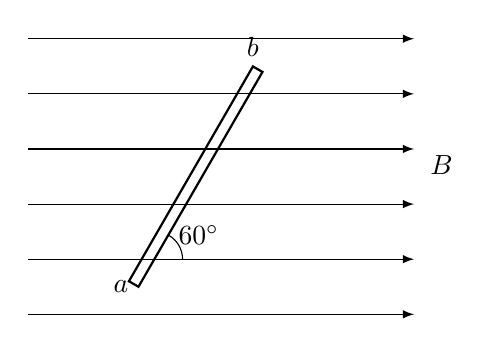
\begin{tikzpicture}[>=latex, scale=.7]
    \foreach \x in {-.5,.5,...,4.5}
    {
       \draw [->](-2,\x)--(5,\x);
    }
    
    \draw [rotate=60, thick](0,0)node [left]{$a$} rectangle (4.5,.2)node [above]{$b$};
    \node at  (5.5,2.2){$B$};
    
    \draw (.8,.5) arc (0:60:.5) node[right]{$60^{\circ}$};
    \end{tikzpicture}
        \caption{}
    \end{figure}
    


    \begin{solution}
    \[I=\frac{F}{\ell B\sin\theta}=\frac{1.0\x 10^{-2}}{0.08\x 4.0\x 10^{-2}\x \frac{\sqrt{3}}{2}}\approx 3.6{\rm A}\]
    电流方向由$b$流向$a$. 
    \end{solution}
    
    \item 一根长2米的直导线,通有1安的电流,把它放在$B=0.2$特的匀强磁场中,当导线与磁力线的夹角为$0^\circ$, $30^\circ$和$90^\circ$时,导线所受的安培力分别有多大?

    \begin{solution}
\[F=I\ell B\sin\theta\]
\begin{itemize}
    \item 当$\theta=0^{\circ}$时,$\sin0^{\circ}=0$, 所以$F=0$,
    \item 当$\theta=30^{\circ}$时,$F=1\x2\x0.2x\dfrac{1}{2}=0.2{\rm N}$,
    \item 当$\theta=90^{\circ}$时,$F=1\x2\x0.2\x1=0.4{\rm N}$.
\end{itemize}
    \end{solution}
    
    \item 如课本图1.27所示,在通电长导线的旁边放一个可以自由移动和转动的矩形通电线圈,线圈和导线在同一平面上,它的$a$, $c$两边和导线平行,试讨论一下线圈各边的受力情况,线圈在磁场中将怎样运动?


    \begin{figure}[htp]
        \centering
        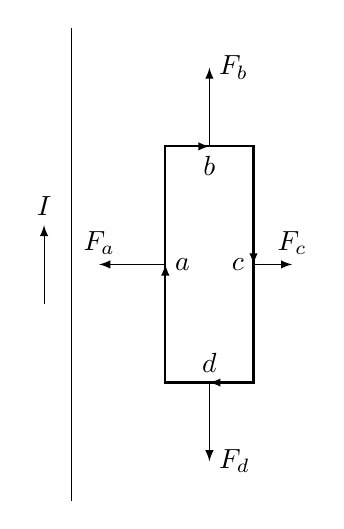
\begin{tikzpicture}[>=latex, xscale=.7]
        \draw (-1,-.5)--(-1,5.5);
        \draw[->] (-1.5,2)--(-1.5,3)node [above]{$I$};
        \draw[thick] (1-.3,1) rectangle (2+.3,4);
        \draw[->] (1-.3,1.5)--(1-.3,2.5)node [right]{$a$};
        \draw [->](2+.3,3)--(2+.3,2.5)node [left]{$c$};
        \draw[->] (1-.3,4)--(1.5,4)node [below]{$b$};
        \draw [->](2+.3,1)--(1.5,1)node [above]{$d$};
        \draw[->](1-.3,2.5)--(-.5,2.5)node[above]{$F_a$};
        \draw[->](2+.3,2.5)--(3,2.5)node[above]{$F_c$};
        \draw[->](1.5,4)--(1.5,4+1)node[right]{$F_b$};
        \draw[->] (1.5,1)--(1.5,0)node[right]{$F_d$};
        \end{tikzpicture}
        \caption{}
        \end{figure}
    \begin{solution}
        根据安培定则可判定线圈所在平面的磁场方向是指
        向纸里.再根据$B\propto \dfrac{1}{r}$
        和左手定则判定出线框各边受的安培
        力方向,即$a$边受的力$F_a$水平向左,$b$边受的力$F_b$竖直向上,
        $c$边受的力$F_c$水平向右,$d$边受的力$F_d$竖直向下,因$F_a>F_c$, $F_b=F_d$, 如图1.26所示,所以矩形线圈将沿着它自己所在的竖直平面向左平动。
    \end{solution}
    
\end{enumerate}




\subsection{练习四}
\begin{enumerate}
    \item 设图1.29所示的长螺线管内部$B=1.0\x10^{-2}$特.
    \begin{enumerate}
        \item 与螺线管轴线平行的一条通电导线所受的力有多大?
        \item 如果$CD$的长度是2厘米,U形导线中通过的电流强度是1.0安,导线所受的力有多大?
        \item 为了使电流天平保持平衡,在另一端要加多重的砝码?
    \end{enumerate}


    \begin{solution}
\begin{enumerate}
    \item 因为电流方向与磁场方向平行,所以$F=0$.
    \item $F=I\ell B=1.0\x0.02\x1.0\x10^{-2}=2\x10^{-4}{\rm N}$
    \item $m=\dfrac{I\ell B}{g}=\dfrac{2\x10^{-4}}{10}=2\x10^{-5}{\rm kg}$
\end{enumerate}

    \end{solution}
    
    \item 你自己设计一种测量磁感应强度的仪器,并说明它的原理和测定方法.

    \begin{solution}
    应用通电导线在磁场中受安培力的原理设计仪器
安培力的大小可通过测量与它平衡的力测出。测量这个与安
培力平衡的力的办法有多种,可使用弹簧秤、天平等仪器。
    \end{solution}
    
\end{enumerate}




\subsection{练习五}
\begin{enumerate}
    \item 如图1.33所示,把通电线圈放入永久磁铁的匀强磁场中.
    \begin{figure}[htp]\centering
  %  	\includegraphics[scale=.75]{fig/1-33.png}
    	\caption{ }
    \end{figure}
    \begin{enumerate}
        \item 图甲中,线圈怎样转动?
        \item 图乙中,由上往下看线圈是顺时针转动的,磁铁哪一边是$N$极?哪一边是$S$极?
        \item 图丙中,由上往下看线圈是反时针转动的,画出线圈中电流的方向.
    \end{enumerate}


    \begin{solution}
    
    \end{solution}
    
    \item 有一个匝数为10匝的矩形线圈,长为25厘米,宽为10厘米,放在$B=1.5\x10^{-3}$特的匀强磁场中,通以1.5安的电流,求它所受的最大的力偶矩.


    \begin{solution}
    
    \end{solution}
    
    \item 图1.30所示的放在磁场中的线圈,当转到线圈平面跟磁力线垂直的位置时,会不会立即停在这个位置上?为什么?定性地分析一下线圈在停下来之前的运动情况,有什么办法可以使通电线圈不停下来而继续转动?


    \begin{solution}
    
    \end{solution}
    
    \item 电流表中通以相同的电流时,指针的偏转角度越大,表示电流表的灵敏度越高,定性地分析一下,有哪些因素会影响磁电式电流表的灵敏度.


    \begin{solution}
    
    \end{solution}
    
\end{enumerate}


\subsection{练习六}

\begin{enumerate}
    \item 如图1.35所示,带电粒子以速率$v$射入匀强磁场.分别标出带电粒子所受洛仑兹力的方向.
    \begin{figure}[htp]\centering
        \begin{tikzpicture}[>=stealth, scale=.5]
    \foreach \x in {1,...,4}
        \foreach \y in {1,...,4}
        {
            \node at (\x,\y){$\times$};
        }
    \draw [->] (-.5,2.5)node [left]{$+q$}--node [below]{$v$}(0.5,2.5);
    \draw (-.5,2.5)[fill=white] circle (3pt);
            \node at (2.5,-1){甲};
        \end{tikzpicture}   \quad 
        \begin{tikzpicture}[>=stealth, scale=.5]
        \foreach \x in {1,...,4}
        \foreach \y in {1,...,4}
        {
            \fill (\x,\y) circle (3pt);
        }
        \draw [->] (-.5,2.5)node [left]{$+q$}--node [below]{$v$}(0.5,2.5);
        \draw (-.5,2.5)[fill=white] circle (3pt);
        \node at (2.5,-1){乙};
        \end{tikzpicture} \quad   \begin{tikzpicture}[>=stealth, scale=.5]
        \foreach \x in {1,...,4}
        {
            \draw [->](\x,0.5)--(\x,4);
        }
        \draw [->] (-.5,2.5)node [left]{$+q$}--node [below]{$v$}(0.5,2.5);
        \draw (-.5,2.5)[fill=white] circle (3pt);
        \node at (2.5,-1){丙};
        \end{tikzpicture} \quad   \begin{tikzpicture}[>=stealth, scale=.5]
        \foreach \x in {1,...,4}
        {
                \draw [<-](\x,0.5)--(\x,4);
        }
        \draw [->] (-.5,2.5)node [left]{$+q$}--node [below]{$v$}(0.5,2.5);
        \draw (-.5,2.5)[fill=white] circle (3pt);
        \node at (2.5,-1){丁};
        \end{tikzpicture}
        \caption{}
    \end{figure}	


    \begin{solution}
    
    \end{solution}
    
    \item 一个带电粒子在空间中运动时没有发生偏转,能不能说明这个空间中没有磁场?为什么?


    \begin{solution}
    
    \end{solution}
    
    \item 一个电子以速率$v$射入磁感应强度为$B$的匀强磁场中,电子沿什么方向射入,受到的洛仑兹力最大?最大值是多大?沿什么方向射入,不受洛仑兹力作用?


    \begin{solution}
    
    \end{solution}
    
    \item 电子的速率$v=3.0\x10^8\ms$,垂直射入$B=0.1$特的磁场中,它受到的洛仑兹力是多大?


    \begin{solution}
    
    \end{solution}
    
    \item 一个电子以$1.2\x10^7\ms$的速率射入磁感应强度为0.02特的匀强磁场中.当速率$v$与磁感应强度$B$的夹角$\theta$为$30^{\circ}$和$60^{\circ}$时,电子所受洛仑兹力分别是多大?


    \begin{solution}
    
    \end{solution}
    
    \item 一电荷$q$在某一匀强磁场中运动,判断下面几种说法是否正确,并说明理由.
\begin{enumerate}
    \item 只要速度的大小相同,所受的洛仑兹力就相同.
    \item 如果速度不变,把电荷$q$改为$-q$,洛仑兹力的方向将反向,但大小不变.
    \item 如果速度不变,把$B$改为反向,洛仑兹力的方向将反向,但大小不变.
\end{enumerate}



\begin{solution}

\end{solution}

\end{enumerate}



 
\subsection{练习七}
\begin{enumerate}
    \item 电子以$1.6\x10^6\ms$的速率垂直射入$B=10^{-4}$特的匀强磁场中,求电子做圆周运动的轨道半径和周期.


    \begin{solution}
    
    \end{solution}
    
    \item 电子垂直射入$B=7.0\x10^{-4}$特的匀强磁场中,做圆周运动的轨道半径为$3.0\x10^{-2}$米,求电子运动的速率.


    \begin{solution}
    
    \end{solution}
    
    \item 能量是5.3兆电子伏的$\alpha$粒子垂直进入磁感应强度是1.0特的匀强磁场中,试确定作用在$\alpha$粒子上的洛仑兹力和$\alpha$粒子的轨道半径.$\alpha$粒子即氦核,质量为$6.6\x10^{-27}$千克,带有两个基本电荷的正电.


    \begin{solution}
    
    \end{solution}
    
    \item 具有相同动能的质子、氘核和$\alpha$粒子垂直进入同一匀强磁场,试比较这些粒子轨道半径的大小,氘核的质量为质子的两倍,带有一个基本电荷的正电.


    \begin{solution}
    
    \end{solution}
    
    \item 两个电子分别以速率$v$和$2v$垂直射入匀强磁场中,经磁场偏转后,哪个电子先回到原来的出发点?


    \begin{solution}
    
    \end{solution}
    
    \item 在匀强磁场中,带电粒子的运动方向不和磁感应强度的方向垂直,它的运动径迹将是什么样的曲线?(只要求定性说明)


    \begin{solution}
    
    \end{solution}
    
\end{enumerate}







\subsection{练习八}
\begin{enumerate}
    \item 在图1.37中,设离子室$A$中产生的是钠离子,加速电压$U=705$伏,磁感应强度$B=3. 85\x10^{-1}$特,$r=5$厘米,求钠离子的荷质比.


    \begin{solution}
    
    \end{solution}
    
    \item 在图1.37所示的装置中,离子从小孔飘出时速度并不相同,因此经加速电场加速后,从缝$S_2$射出时速度也不相同,这对实验有一定影响.于是人们提出在缝$S_2$和$S_3$之间加一个\textbf{速度选择器}(图1.38),其中$D_1$和$D_2$是两个平行金属板,分别连在电源的两极上,其间有一定的电场强度$E$;同时在这空间加有垂直于电场方向的磁场,磁感应强度为$B$.这时具有一定速度的带电粒子,从缝$S_2$垂直进入后,可以不发生偏转,由缝$S_2$射出;而具
有其他速度的带电粒子都发生偏转,不能由缝$S_2$射出,为什么?这个一定的速度$v$有多大?
\begin{figure}[htp]\centering
	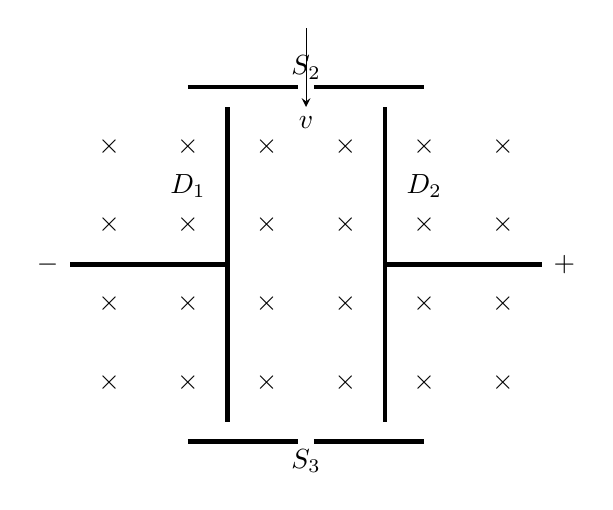
\begin{tikzpicture}[>=stealth, scale=1]
	\foreach \x in {1,...,6}
	\foreach \y in {1,...,4}
	{
		\node at (\x,\y){$\times$};
	}

\draw [ultra thick] (2.5,0.5)--(2.5,4.5)	;
\draw [ultra thick] (4.5,0.5)--(4.5,4.5)	;
\draw  [ultra thick](2.5,2.5)--(0.5,2.5)node [left]{$-$};
\draw  [ultra thick](4.5,2.5)--(6.5,2.5)node [right]{$+$};

\draw [ultra thick] (2,4.75)--(3.4,4.75);  \draw  [ultra thick](3.6,4.75)--(5,4.75);
\draw  [ultra thick](2,.25)--(3.4,.25);  \draw  [ultra thick](3.6,.25)--(5,.25);
\draw [->](3.5, 5.5)--(3.5, 4.5) node [below]{$v$};
\node at (3.5,5){$S_2$};\node at (3.5,0){$S_3$};
\node at (2,3.5){$D_1$};\node at (5,3.5){$D_2$};

	\end{tikzpicture}
	\caption{速度选择器的原理示意图}
\end{figure}


\begin{solution}

\end{solution}

\item 带电粒子带正电或者带负电,会不会影响速度选择器对它们的速度的选择?如果把图1.38中的电场方向改变为相反的方向,或者把磁场方向改变为相反的方向,速度选择器还能不能使用?如果把电场和磁场同时改变为相反的方向,还能不能使用?


\begin{solution}

\end{solution}

\end{enumerate}





\subsection{习题}
\begin{enumerate}
    \item 照图1.42那样,把一根柔软的弹簧竖直地悬挂起来,使它的下端刚刚跟导电液体接触,给弹簧通入电流时,会发生什么现象?做一下这个实验,并解释所发生的现象.

\begin{figure}[htp]
\centering
\begin{minipage}[t]{0.48\textwidth}
\centering
   % 	\includegraphics[scale=.75]{fig/1-42.png}
\caption{}
\end{minipage}
\begin{minipage}[t]{0.48\textwidth}
\centering
	%\includegraphics[scale=.75]{fig/1-43.png}
\caption{}
\end{minipage}
\end{figure}



\begin{solution}

\end{solution}

    \item 把一个可以绕水平轴转动的铝盘放在蹄形磁铁之间,盘的下边缘浸在导电液体中(图1.43).把转轴和导电液体分别接到直流电源的两极上,铝盘就会转动起来.为什么?用什么方法可以改变铝盘的转动方向?


    \begin{solution}
    
    \end{solution}
    
\item 在玻璃皿中放入电解质溶液,在玻璃皿的中心放一个圆柱形电极,边缘放一个围环形电极,分别接在电池的两极
上(图1.44),如果把玻璃里放在磁场中,液体就旋转起来.为什么?液体旋转的方向跟什么有关系?做一下这个实验,看你的判断是否正确?
\begin{figure}[htp]\centering
	%\includegraphics[scale=.75]{fig/1-44.png}
	\caption{ }
\end{figure}


\begin{solution}

\end{solution}

\item 下列说法中,哪些说法是正确的?
\begin{enumerate}
    \item 一小段通电导线放在磁感应强度为零的位置,所受的安培力一定等于零.
    \item 一小段通电导线在磁场中某点不受磁场力的作用,该点的磁感应强度一定为零.
    \item 一小段通电导线在磁场中所受安培力的方向、该点的磁感应强度的方向、电流的方向三者一定互
相垂直.
\end{enumerate}



\begin{solution}

\end{solution}

\item 磁电式电流表中的磁场是均匀地辐向分布的,线圈两侧边所在位置的磁感应强度为0.02特.线圈是边长1厘米的正方形,共100匝,线圈每转$1^{\circ}$,螺旋弹簧产生阻碍线圈偏转的力矩是$2.5\x10^{-8}{\rm N}\cdot {\rm m}$.线圈中电流强度为5毫安时,指针将偏转多少度?


\begin{solution}

\end{solution}

\item 洛仑兹力对带电粒子是否做功?为什么?    


\begin{solution}

\end{solution}

\item 利用学过的知识,想办法把下面的带电粒子分开:
\begin{enumerate}
    \item 速度分别为$v$和$3v$的电子;
    \item 具有相同动能的质子和$\alpha$粒子;
    \item 荷质比不同的带正电的粒子.
\end{enumerate}

\begin{figure}[htp]
\centering
\begin{minipage}[t]{0.48\textwidth}
\centering
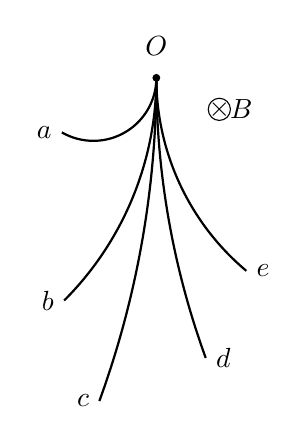
\begin{tikzpicture}[>=latex, scale=.8]
\draw [thick](0,0) arc (0:-120:1)node[left]{$a$};
\draw [thick](0,0) arc (0:-45:5)node[left]{$b$};
\draw [thick](0,0) arc (0:-20:15)node[left]{$c$};
\draw[thick] (0,0) arc (180:200:13)node[right]{$d$};
\draw [thick](0,0) arc (180:230:4)node[right]{$e$};
\draw (1,-.5) [fill=white] circle (5pt);
\node at (1,-.5){$\times$};
\node at (1.35,-.5){$B$};
\node at (0,.5){$O$};
\draw (0,0) [fill=black] circle (1.5pt);

\end{tikzpicture}
\caption{}
\end{minipage}
\begin{minipage}[t]{0.48\textwidth}
\centering
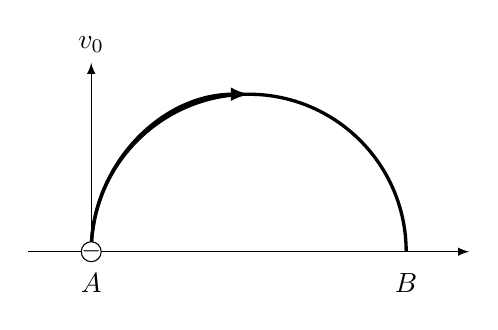
\begin{tikzpicture}[>=latex, scale=.8]
\draw[->] (-1,0)--(6,0);
\draw[->] (0,0)--(0,3)node [above]{$v_0$};
\draw[very thick] (0,0) arc (180:0:2.5); 
\draw[very thick, ->] (0,0) arc (180:90:2.5); 
\node at (0,-.5){$A$};\node at (5,-.5){$B$};

\draw (0,0) [fill=white]circle (4.5pt);
\node at  (0,0) {\small $-$};


\end{tikzpicture}
\caption{}
\end{minipage}
\end{figure}



\begin{solution}

\end{solution}


\item 图1.45表示由$O$点发出的电子和正电子(质量和电量跟电子相同,但带的是正电荷)在匀强磁场中运动的径迹.
哪些径迹是电子的,哪些径迹是正电子的?$a$, $b$, $c$三条径迹中,哪个粒子的能量最大,哪个最小?


\begin{solution}

\end{solution}

\item 质子、氘核和$\alpha$粒子由静止开始通过相同的电势差后垂直进入同一匀强磁场.
\begin{enumerate}
    \item 比较这些粒子的动能.
    \item 如果质子在磁场中的轨道半径为10厘米,氘核和$\alpha$粒子的轨道半径各有多大?
\end{enumerate}


\begin{solution}

\end{solution}

\item 如图1.46所示,$A$和$B$之间的距离为0.1米,位于$A$点的电子的速度$v_0=1.0\x10^7\ms$.
\begin{enumerate}
    \item 要使电子沿半圆周由$A$运动到$B$,求磁感应强度的大小和方向.
    \item 电子从$A$
运动到$B$需要多长时间?
\end{enumerate}


\begin{solution}

\end{solution}

\item 把图1.38所示的速度选择器加在图1.37所示装置的$S_2$和$S_3$之间,已知速度选择器的电场强度为$E$,磁感应强度为$B_1$.粒子从缝$S_3$进入磁感应强度为$B_2$的匀强磁场中,做圆周运动的半径为$r$.求粒子的荷质比.


\begin{solution}

\end{solution}

\item  有一回旋加速器,它的交变电压的频率为$12\x10^8$赫,半圆形电极的半径为0.53米.加速氘核所需的磁感应强
度要多大?氘核的最大动能是多大?已知氘核的质量为$3.3\x10^{-27}$千克,电量为$1.6\x10^{-19}$库.


\begin{solution}

\end{solution}

\item 目前世界上正在研究一种新型发电机,叫做磁流体发电机,它可以把气体的内能直接转化为电能.图1.47表示出了它的发电原理:将一束等离子体(即高温下电离的气体,含有大量带正电和带负电的微粒,但从总体来说呈中性),喷射入磁场,磁场中有两块金属板1和2,这时金属板上就会集聚电荷,产生电压,说明金属放上为什么会聚集电荷.在磁极配置如图中所示的情况下,电路中的电流方向如何?

磁流体发电是一项新兴技术,报纸、杂志上常有文章介
绍,希望有兴趣的同学找来看看,以扩展自己的知识面.


\begin{solution}

\end{solution}

\item  图1.48表示两个平行金属板,它们之间的距离为$d$,分别接在电源的两极上.在两平行金属板当中的空间存在着彼此垂直的电场和磁场,电场强度为$E$,磁感应强度为$B$. 从负极板的小孔射入一个电子,经过有电场和磁场同时存在的空间,并打在正极板上,射入电子的初速度为$v0$,方向跟竖直方向成$\theta$角.求电子打在正极板上的速度的大小.

\begin{figure}[htp]\centering
%	\includegraphics[scale=.75]{fig/1-47.png}
	\caption{ }
\end{figure}\begin{figure}[htp]\centering
%\includegraphics[scale=.75]{fig/1-48.png}
\caption{ }
\end{figure}


\begin{solution}

\end{solution}

\end{enumerate}



















